\documentclass[12pt, a4 paper]{article}
\usepackage[T2A]{fontenc}
\usepackage[utf8]{inputenc}
\usepackage[russian,english]{babel}
\usepackage{amsmath,amssymb,amsfonts,amsthm}
\usepackage{indentfirst}
\usepackage{titlesec}
\usepackage{graphicx}
\usepackage{setspace}

\titleformat*{\section}{\Large\bfseries\filcenter}
\titleformat*{\subsection}{\large\bfseries\filcenter}
\titleformat*{\subsubsection}{\normalsize\bfseries\filcenter}

\usepackage{cmap}                   % поиск в PDF

\usepackage{geometry}
    \geometry{top=20mm}
    \geometry{bottom=20mm}
    \geometry{left=30mm}
    \geometry{right=15mm}		

\begin{document}
\selectlanguage{russian}


\section{Численные расчёты}
\subsection{Простейшие случаи}

Рассмотрим работу процедуры в простейших случаях на данном примере:

\begin{figure}[h]
  \begin{center}
      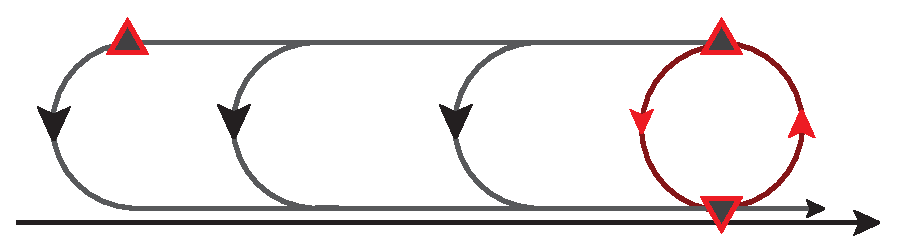
\includegraphics[scale=0.8]{StandardScheme.eps}%MaketTest.png
        \caption{Макетный пример}                                                                             
  \end{center}
\end{figure}

Пусть расстояние будет в метрах, а скорость в метрах в секунду.

\noindent Файл с данными точек:\\
9\\
a -100 0 0 5 10\\
b -50 0 0 5 10\\
c 0 0 0 5 10\\
d 50 0 0 5 10\\
e 200 0 0 4 6\\
f 50 100 0 4 8\\
g -50 50 0 5 10\\
h -200 50 0 5 10\\
r 400 0 0 2 5 LAND\\

\noindent Файл с данными схем:\\
3\\
1\\
Name1 (e)(r):\\
Name2 (a)(e): a Str(f) b c d /Str f e\\
NameSt1 (0): b g h\\

\noindent Файл с данными потоков:\\
3\\
Flow1 e\\
Flow2 a\\

\subsubsection{Движение по прямой}


Рассмотрим движение по прямой на примере первого потока:


$$
T_{min} = \frac{2S}{v_{max}^e + v_{max}^r} = \frac{2\cdot\sqrt{(400 - 200)^2}}{6 + 5} \approx 36.(36) ~sec
$$

$$
T_{max} = \frac{2S}{v_{min}^e + v_{min}^r} = \frac{2\cdot\sqrt{(400 - 200)^2}}{4 + 2} \approx 66.(66) ~sec
$$

И результат процедуры:

\noindent Flow1:\\
e $\rightarrow$ [0~sec, 0~sec]\\
r $\rightarrow$ [36.36~sec, 66.67~sec]


%---------------------------------------------------------------------------------

\subsubsection{Движение по вееру и прямым участкам}

Движение по вееру и прямым участкам рассмотрим на примере второго потока. Рассчитаем временной интервал для точки $f$:


\begin{eqnarray*}

T_{min} = \frac{2S_{a-b}}{v_{max}^b + v_{max}^a} + \frac{2S_{b-f}}{v_{max}^f + v_{max}^b}
= \frac{2\cdot\sqrt{(-50 + 100)^2}}{10 + 10} + \frac{2\cdot\sqrt{(50 + 50)^2 + (100-0)^2}}{8 + 10} \approx 20.71348 ~sec

\end{eqnarray*}

\begin{eqnarray*}

T_{max} = T_{max}^{a-b} + T_{max}^{b-c} + T_{max}^{c-d} + T_{max}^{d-f} = 
 \frac{2S_{a-b}}{v_{min}^b + v_{min}^a} + \frac{2S_{b-c}}{v_{min}^c + v_{min}^b} +
 \frac{2S_{c-d}}{v_{min}^d + v_{min}^c} + \frac{2S_{d-f}}{v_{min}^f + v_{min}^d} =
 \frac{2\cdot\sqrt{(-50 + 100)^2}}{5 + 5} + \frac{2\cdot\sqrt{(0 + 50)^2}}{5 + 5} +
 \frac{2\cdot\sqrt{(50 - 0)^2}}{5 + 5} + \frac{2\cdot\sqrt{(50 - 50)^2 + (100-0)^2}}{5 + 4}
 = 10 + 10 + 10 + 22.(2) = 52.(2) ~sec

\end{eqnarray*}


Результат процедуры:
Flow2:\\
a $\rightarrow$ [0 sec, 0 sec]\\
b $\rightarrow$ [5 sec, 10 sec]\\
c $\rightarrow$ [10 sec, 20 sec]\\
d $\rightarrow$ [15 sec, 30 sec]\\
f $\rightarrow$ [20.71 sec, 52.22 sec]\\
e $\rightarrow$ [46.47 sec, 97.29 sec]\\
r $\rightarrow$ [82.83 sec, 163.96 sec]\\


%---------------------------------------------------------------------------------

\subsubsection{Движение по вееру и прямым участкам со стандартной схемой}

Теперь изменим файл схем следующим образом --- добавим одно повторение к стандартной схеме:

\noindent 3\\
1\\
Name1 (e)(r):\\
Name2 (a)(e): a Str(f) b c d /Str f e\\
NameSt1 \underline{(1)}: b g h

И запустим поток с точки a:

\noindent 1\\
Flow1 a

Посчитаем время минимальной и максимальной задержки на <<тромбоне>>:

Вычислим радиус поворота, как половину от расстояния между b и g:

$$
 R = \frac{1}{2} \cdot \sqrt{(-50 + 50)^2 + (50 - 0)^2} = 25
$$

Длину плеча найдём, как расстояние между h и g:

$$
S = \sqrt{(-200 + 50)^2 + (50 - 50)^2} = 150
$$

$$
T_{min} = \frac{2 \pi R}{v_{max}^b} = \frac{2 \pi \cdot 25}{10} = 5\pi \approx 15.7
$$

$$
T_{max} = \frac{2(S + \pi R)}{v_{min}^b} = \frac{2(150 + \pi \cdot 25)}{5} = 60 + 10\pi \approx 91.4
$$

Результат процедуры:

\noindent Flow1:\\
a $\rightarrow$ [0 sec, 0 sec]\\
b $\rightarrow$ [5 sec, 10 sec] [20.71 sec, 101.42 sec]\\
c $\rightarrow$ [10 sec, 20 sec] [25.71 sec, 111.42 sec]\\
d $\rightarrow$ [15 sec, 30 sec] [30.71 sec, 121.42 sec]\\
f $\rightarrow$ [20.71 sec, 143.64 sec]\\
e $\rightarrow$ [46.47 sec, 188.71 sec]\\
r $\rightarrow$ [82.83 sec, 255.37 sec]\\


Как можно заметить, появился новый временной интервал соответствующий проходу по стандартной схеме.

\newpage

%======================================================================


\subsection{Расчёты для аэропорта <<Кольцово>>}

Рассмотрим работу программы на примере аэропорта Кольцово.

Общий вид зоны Кольцово представлен на рис.~\ref{KoltsAll}. Вид внутренней зоны представлен на рис.~ \ref{KoltsLand}

\begin{figure}[h]
  \begin{center}
      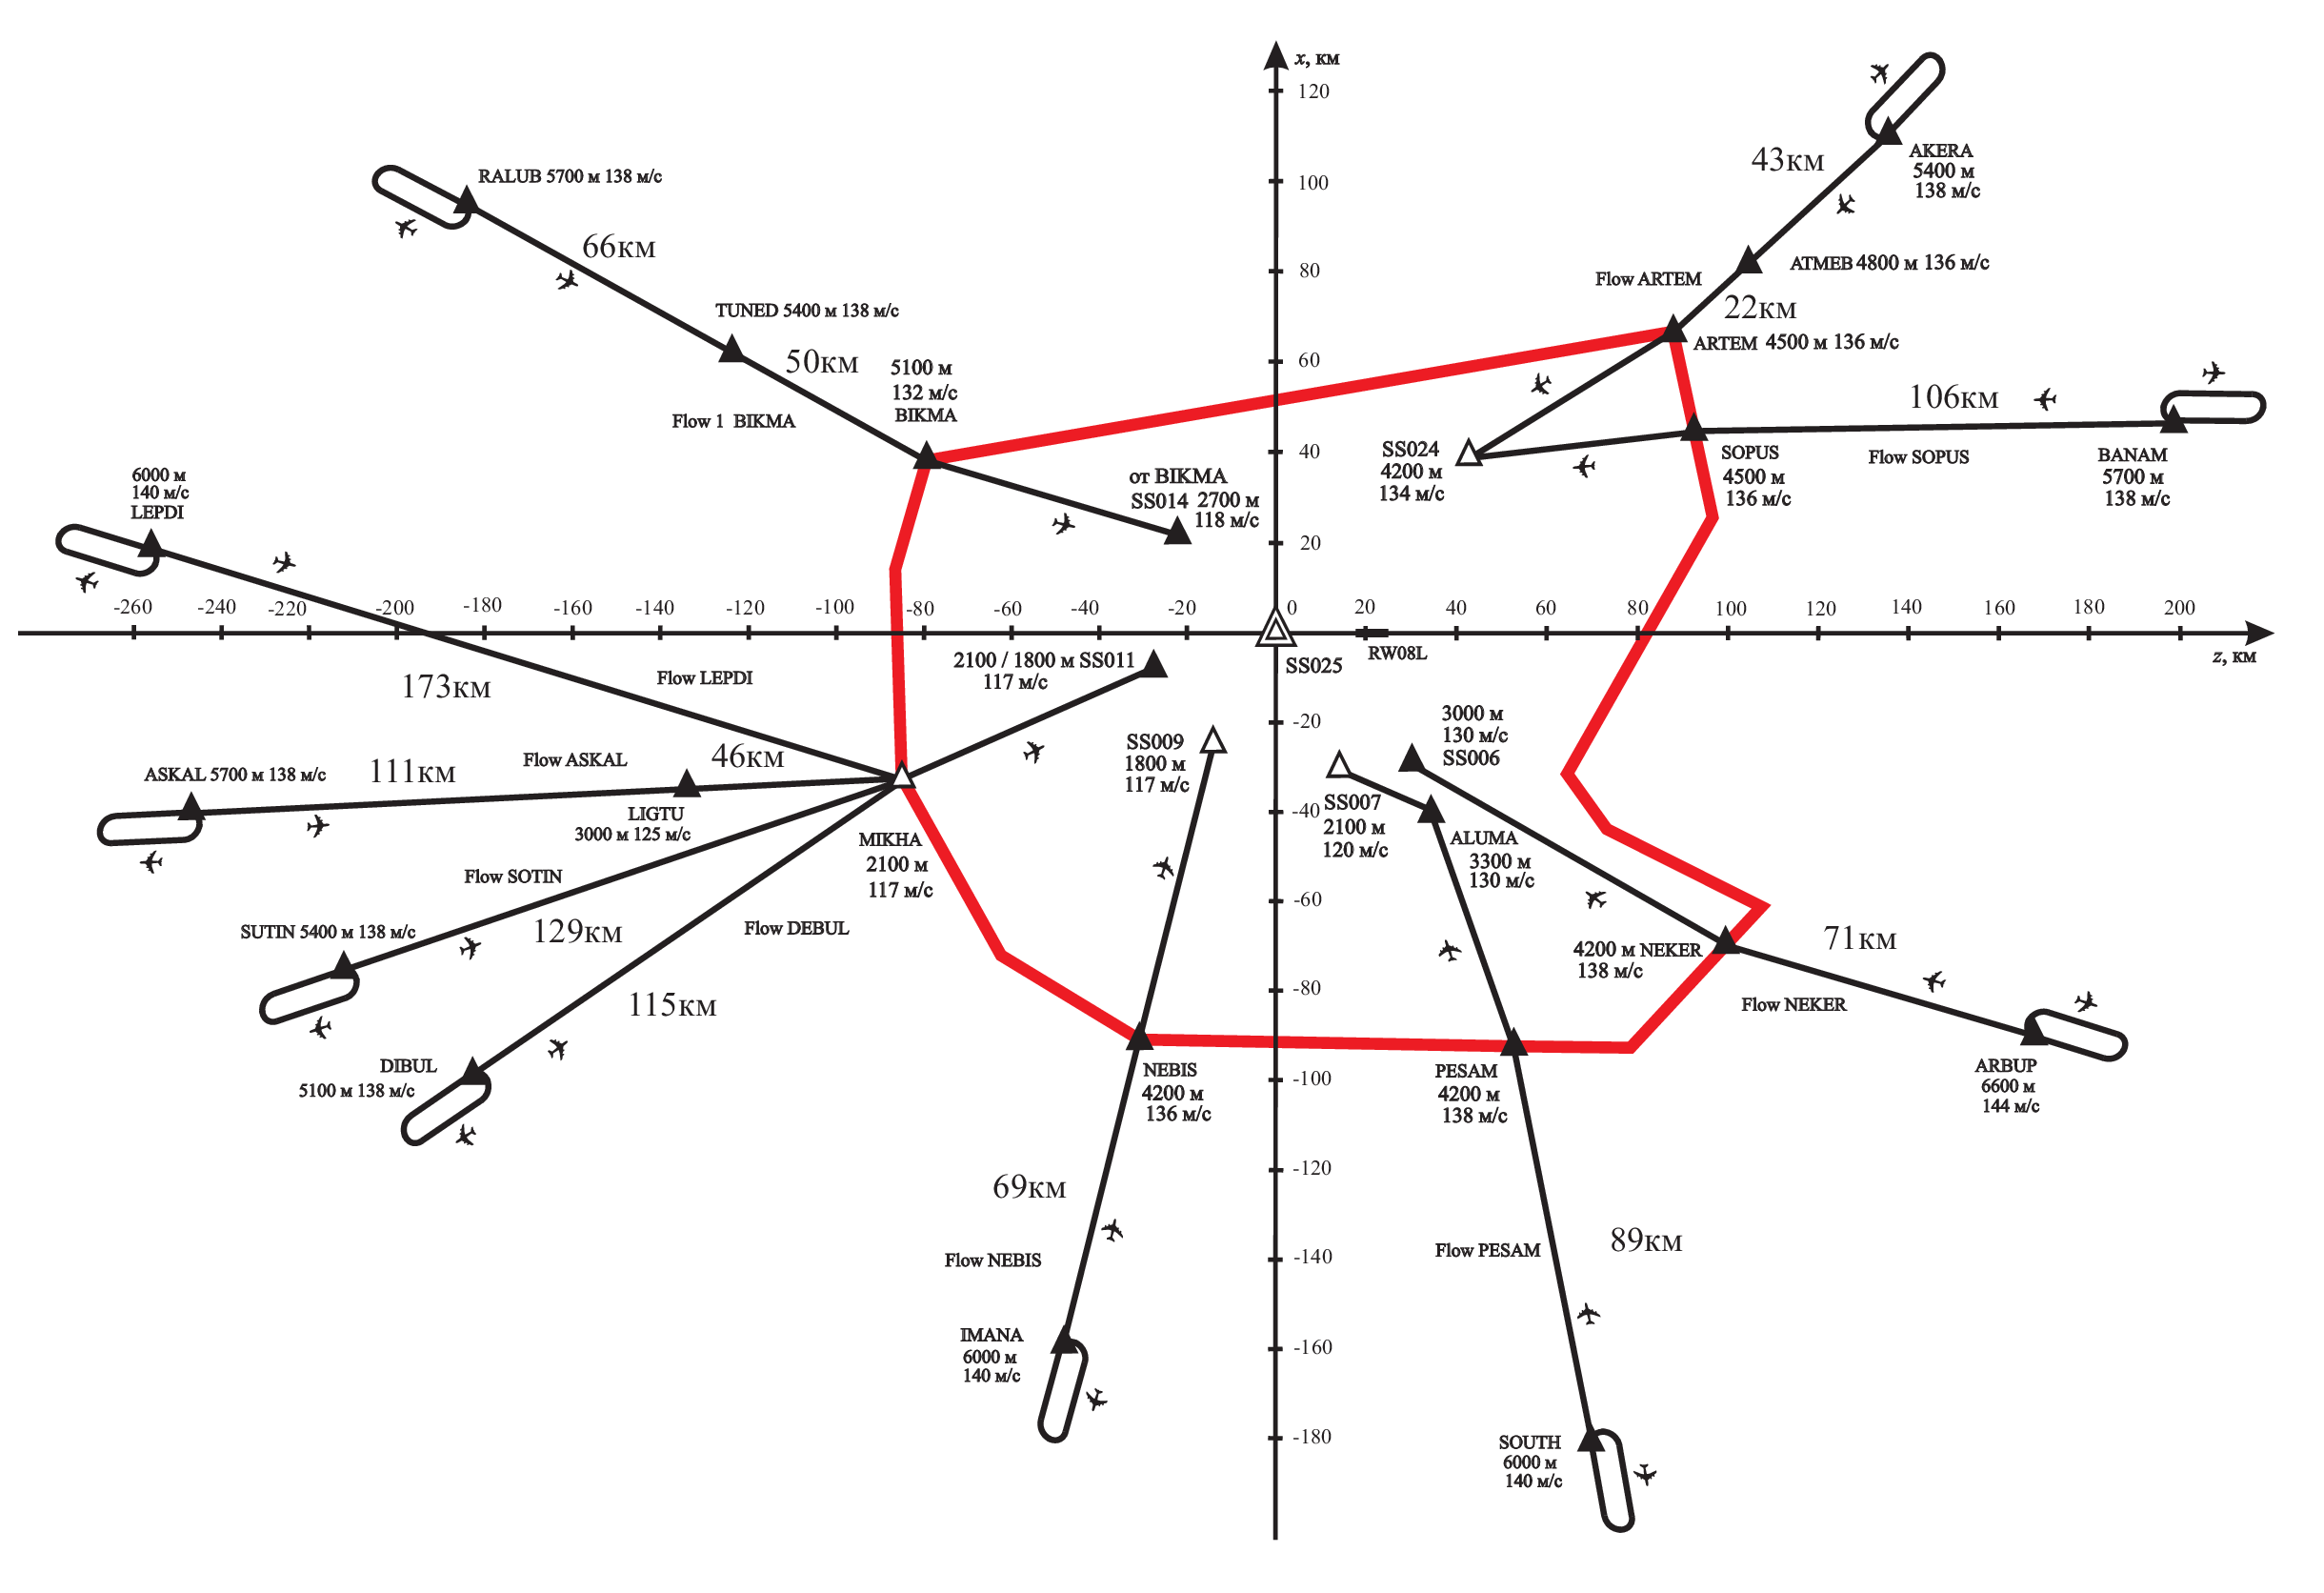
\includegraphics[scale=0.25]{Koltsovo01.png}
        \caption{Общий вид зоны Кольцово}                                                                             
    \label{KoltsAll}
  \end{center}
\end{figure}

\begin{figure}[h]
  \begin{center}
      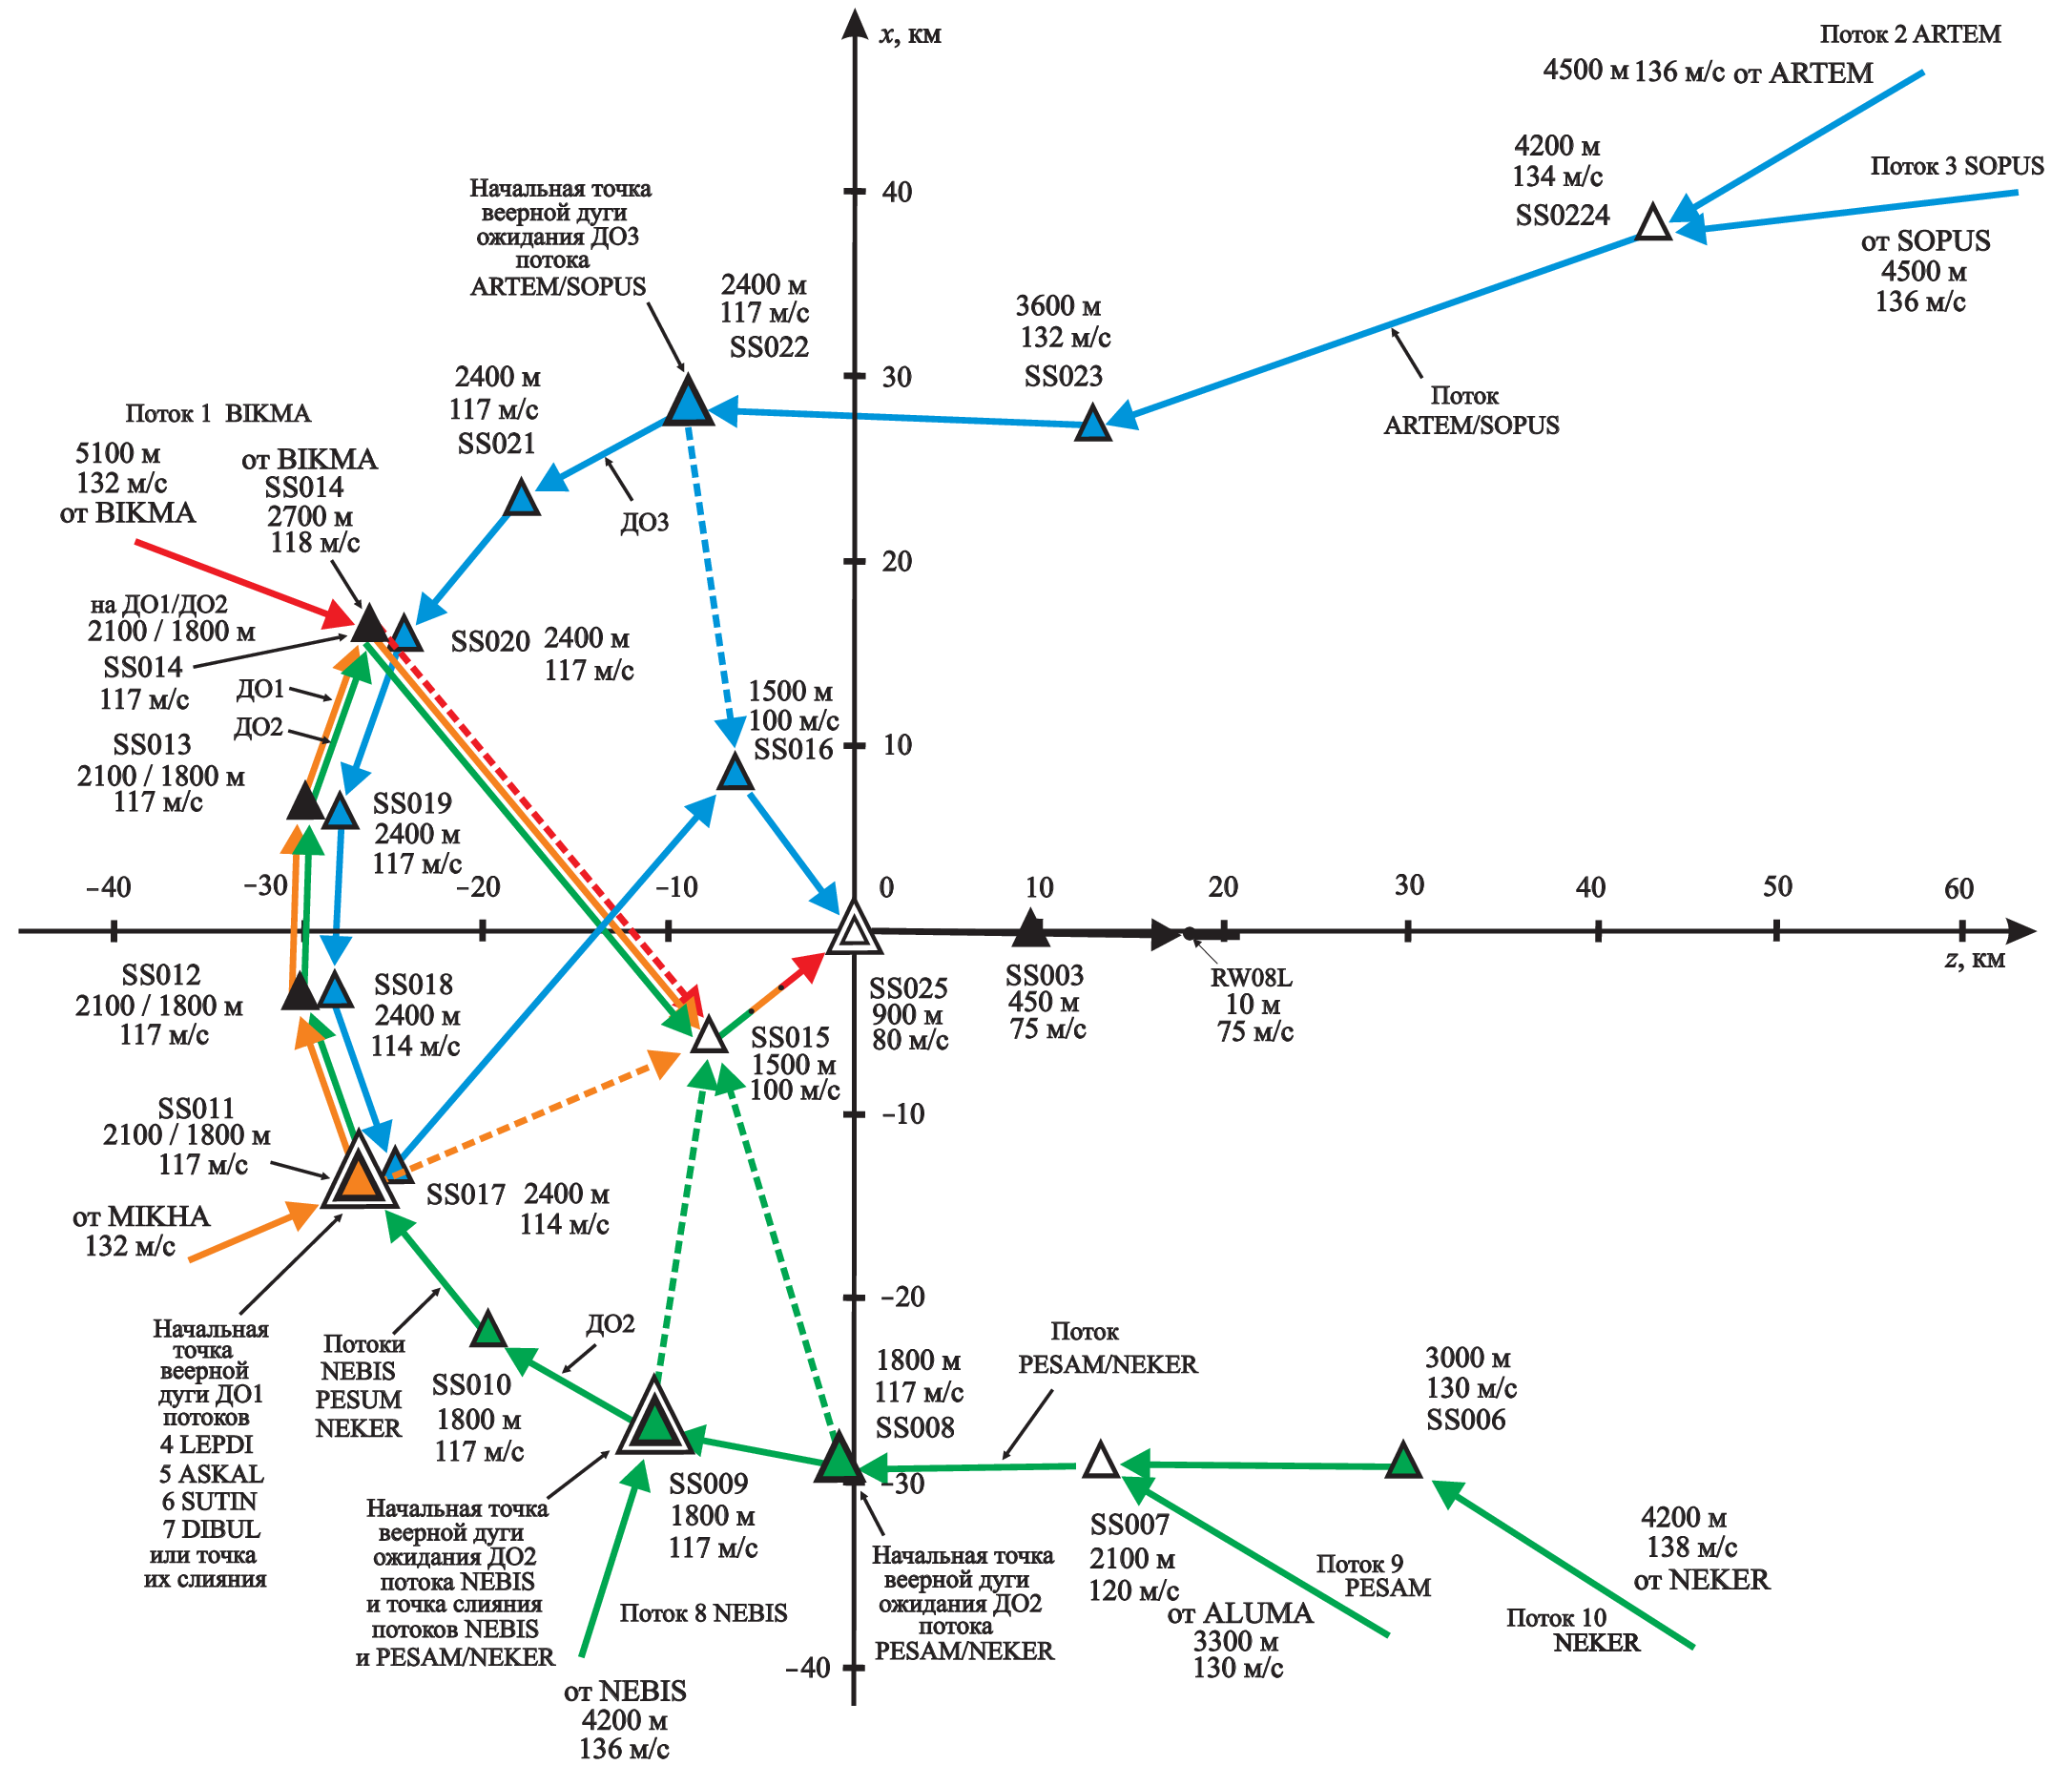
\includegraphics[scale=0.25]{Koltsovo02.png}
        \caption{Прибывающие потоки и веерные схемы их слияния.}                                                                             
    \label{KoltsLand} 
  \end{center}
\end{figure}

Рассмотрим поток BIKMA начинающийся в точке RALUB.

Результаты работы процедуры для потока BIKMA c нулём повторений стандартной схемы:

\noindent Flow1BIKMA:\\
RALUB $\rightarrow$ [0 sec, 0 sec]\\
TUNED $\rightarrow$ [474.52 sec, 548.67 sec]\\
BIKMA $\rightarrow$ [818.27 sec, 947.42 sec]\\
SS014 $\rightarrow$ [1240.52 sec, 1443.1 sec]\\
SS015 $\rightarrow$ [1482.57 sec, 1734.04 sec]\\
SS025 $\rightarrow$ [1578.33 sec, 1853.75 sec]\\
SS003 $\rightarrow$ [1684.27 sec, 1991.08 sec]\\
RW08L $\rightarrow$ [1792.31 sec, 2132.36 sec]\\


Результаты работы процедуры для потока BIKMA c однократным повторением стандартной схемы:

\noindent Flow1BIKMA:\\
RALUB $\rightarrow$ [0 sec, 0 sec] [389.33 sec, 992.17 sec]\\
TUNED $\rightarrow$ [474.52 sec, 548.67 sec] [863.86 sec, 1540.84 sec]\\
BIKMA $\rightarrow$ [818.27 sec, 947.42 sec] [1207.61 sec, 1939.58 sec]\\
SS014 $\rightarrow$ [1240.52 sec, 1443.1 sec] [1629.85 sec, 2435.26 sec]\\
SS015 $\rightarrow$ [1482.57 sec, 1734.04 sec] [1871.9 sec, 2726.21 sec]\\
SS025 $\rightarrow$ [1578.33 sec, 1853.75 sec] [1967.66 sec, 2845.91 sec]\\
SS003 $\rightarrow$ [1684.27 sec, 1991.08 sec] [2073.6 sec, 2983.24 sec]\\
RW08L $\rightarrow$ [1792.31 sec, 2132.36 sec] [2181.64 sec, 3124.52 sec]\\


Рассмотрим поток NEKER начинающийся в точке ARBUP.

Результаты работы процедуры для потока NEKER c нулём повторений стандартной схемы:

\noindent Flow10NEKER:\\
ARBUP $\rightarrow$ [0 sec, 0 sec]\\
NEKER $\rightarrow$ [463.24 sec, 533.96 sec]\\
SS006 $\rightarrow$ [1015.68 sec, 1175.5 sec]\\
SS007 $\rightarrow$ [1140.14 sec, 1321.61 sec]\\
SS008 $\rightarrow$ [1249.54 sec, 1451.18 sec]\\
SS009 $\rightarrow$ [1331.5 sec, 1548.45 sec]\\
SS010 $\rightarrow$ [1413.66 sec, 1645.98 sec]\\
SS011a $\rightarrow$ [1496.1 sec, 1743.82 sec]\\
SS012a $\rightarrow$ [1578.68 sec, 1841.84 sec]\\
SS013a $\rightarrow$ [1661.3 sec, 1939.91 sec]\\
SS014aaa $\rightarrow$ [1743.95 sec, 2038 sec]\\
SS015 $\rightarrow$ [1455.79 sec, 2330.19 sec]\\
SS025 $\rightarrow$ [1551.56 sec, 2449.89 sec]\\
SS003 $\rightarrow$ [1657.5 sec, 2587.22 sec]\\
RW08L $\rightarrow$ [1765.54 sec, 2728.5 sec]\\



Результаты работы процедуры для потока NEKKER c однократным повторением стандартной схемы в точке ARBUP:

\noindent Flow10NEKER:\\
ARBUP $\rightarrow$ [0 sec, 0 sec] [234.91 sec, 925.33 sec]\\
NEKER $\rightarrow$ [463.24 sec, 533.96 sec] [698.15 sec, 1459.29 sec]\\
SS006 $\rightarrow$ [1015.68 sec, 1175.5 sec] [1250.59 sec, 2100.83 sec]\\
SS007 $\rightarrow$ [1140.14 sec, 1321.61 sec] [1375.04 sec, 2246.93 sec]\\
SS008 $\rightarrow$ [1249.54 sec, 1451.18 sec] [1484.45 sec, 2376.51 sec]\\
SS009 $\rightarrow$ [1331.5 sec, 1548.45 sec] [1566.4 sec, 2473.78 sec]\\
SS010 $\rightarrow$ [1413.66 sec, 1645.98 sec] [1648.57 sec, 2571.31 sec]\\
SS011a $\rightarrow$ [1496.1 sec, 2669.15 sec]\\
SS012a $\rightarrow$ [1578.68 sec, 2767.16 sec]\\
SS013a $\rightarrow$ [1661.3 sec, 2865.24 sec]\\
SS014aaa $\rightarrow$ [1743.95 sec, 2963.33 sec]\\
SS015 $\rightarrow$ [1455.79 sec, 3255.51 sec]\\
SS025 $\rightarrow$ [1551.56 sec, 3375.21 sec]\\
SS003 $\rightarrow$ [1657.5 sec, 3512.54 sec]\\
RW08L $\rightarrow$ [1765.54 sec, 3653.83 sec]\\



\end{document}